%\documentclass[a4paper,12pt]{article}%正文小四
\documentclass[a4paper,12pt,UTF8]{ctexart}
\usepackage{color}
\usepackage{geometry}
\usepackage{authblk}
\usepackage{setspace}
\usepackage[english]{babel}
\usepackage[T1]{fontenc}
\usepackage{fancyhdr}
\usepackage{graphicx}
\usepackage{titlesec} 
\usepackage{titletoc}  
\usepackage{pdfpages}
\usepackage{hyperref} 
\usepackage{booktabs} 
\usepackage{amsmath}
\usepackage{amssymb}
\usepackage{dsfont}
\usepackage{algorithm}
\usepackage{algorithmicx}
\usepackage[noend]{algpseudocode}
\usepackage{bm}  
\usepackage{paralist}
\usepackage{enumitem}
\usepackage{pdfpages}
\usepackage{hyperref}
\usepackage{longtable}
\usepackage{framed}
\usepackage{ragged2e}
\usepackage{textcomp}
\usepackage{stmaryrd}
\usepackage{tikz}
\usepackage{verbatim}

\geometry{left=3.17cm, right=3.17cm,top=2.54cm,bottom=2.54cm}
\setlength{\textheight}{24cm}  
\pagenumbering{arabic}
\pagestyle{fancy}                    % 设置页眉                                                
\lhead{\small Bachelor's Thesis of Northeastern University}                                                                  
                                               
\cfoot{\thepage}                                                                       
\renewcommand{\headrulewidth}{1pt}  %页眉线宽,设为0可以去页眉线
\setlength{\headheight}{0.9cm}     %页眉距边界1.5cm 2.54-1.04
\renewcommand{\footnotesize}{}      %设置脚注字体大小           
\renewcommand{\footrulewidth}{0pt}  %脚注线的宽度 
\setlength{\topskip}{0cm} 
\renewcommand{\labelitemi}{$\vcenter{\hbox{\tiny$\bullet$}}$}
\graphicspath{ {fig/} }
\titleformat{\section}%设置一级标题的样式
{\raggedright\LARGE\bfseries}%右对齐,2号字,黑体
{\thesection.\quad}%标号后面有个点
{0pt}%sep label和title之间的水平距离
{}%标题前没有内容
\titleformat{\subsection}%设置二级标题的样式
{\raggedright\Large\bfseries}%右对齐,3号字,黑体
{\thesubsection.\quad}%标号后面有个点
{0pt}%sep label和title之间的水平距离
{}%标题前没有内容
\titleformat{\subsubsection}%设置三级标题的样式
{\raggedright\large\bfseries}%右对齐,4号,黑体
{\thesubsubsection.\quad}%标号后面有个点
{0pt}%sep label和title之间的水平距离
{}%标题前没有内容
\hyphenpenalty=5000 %值越大,断字越少
\tolerance=1000 %tolerance越大,换行就会越少
\justifying
\makeatletter
\newcommand{\rmnum}[1]{\romannumeral #1}
\newcommand{\Rmnum}[1]{\expandafter\@slowromancap\romannumeral #1@}
\renewcommand {\thetable} {\thesection{}.\arabic{table}}
\renewcommand {\thefigure} {\thesection{}.\arabic{figure}}
\renewcommand{\theequation}{\arabic{section}.\arabic{equation}}
\makeatother
\begin{document}
	
\date{}

\includepdf{cover1.pdf}
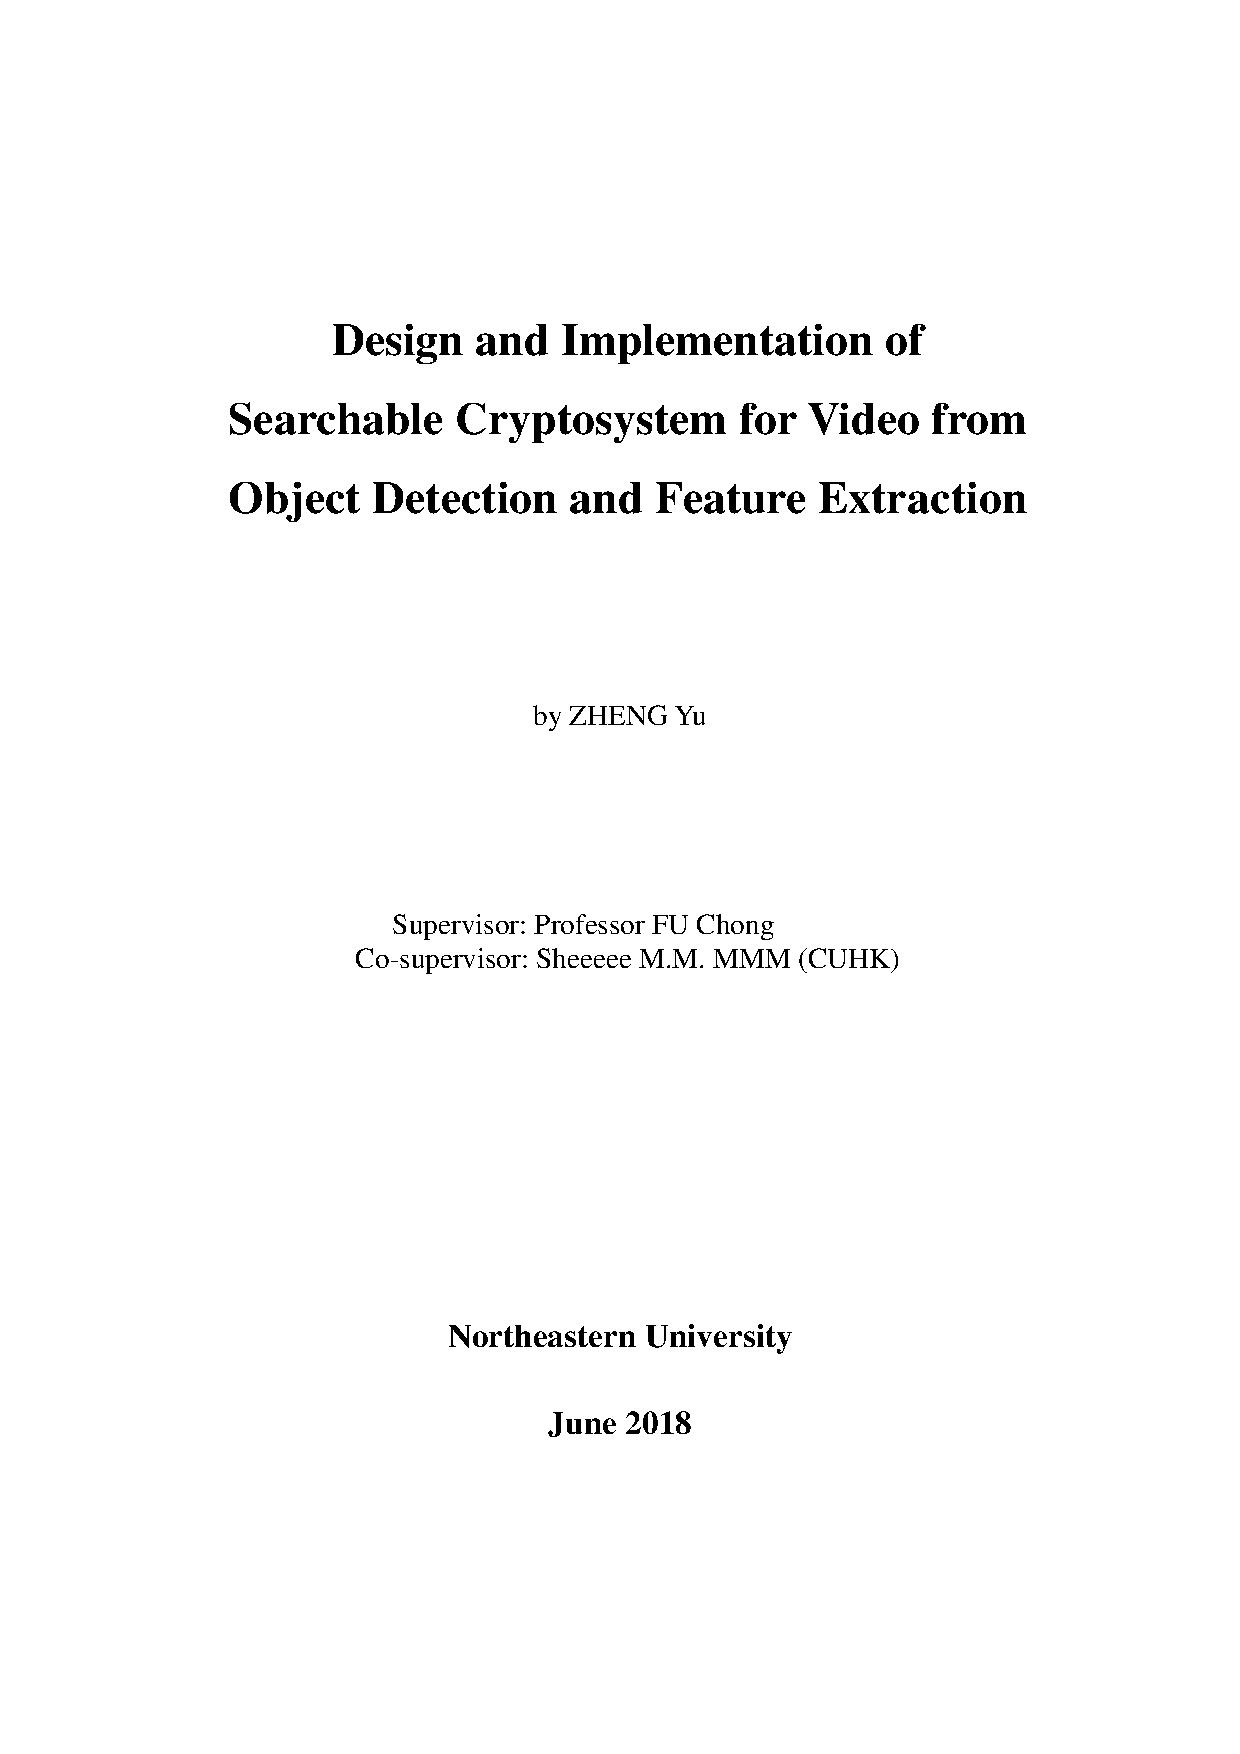
\includepdf{cover2.pdf}  %封面我用的插入pdf 这个文档里的word模板改完导出pdf插入就可以
%\addcontentsline{toc}{section}{Proposal}  %该命令还有其他可选参数请自行百度,该命令可以在目录里自行添加行. 但是例子里没有因为忘记改了2333333
\clearpage
\rhead{\small 任务书}   
\pagenumbering{Roman}
\begin{figure}[t]
	\centering
	
\includegraphics[width=1\textwidth]{proposal.png} %由于时间关系,任务书是图片格式,有一个Adobe acrobat X的软件,可以免费用30天,缺点是比较大,可以毕设提交之前下载,也可以用插入pdf,插入pdf会有页码编码问题,我选了比较省事的图片,有时间有能力的学弟学妹可以自己用latex画一个。
\end{figure}
%\addcontentsline{toc}{section}{Abstract (Chinese)}
\clearpage
\rhead{\small 摘要} 
\begin{spacing}{1.35}
	\begin{center}
		\large
		\textbf{致学弟学妹}
	\end{center}
\indent\indent 学弟学妹们好,我是14级学姐郑宇,这是我第一次尝试搭建latex模板也是第一次使用Latex,非常拙劣简单,还有很多瑕疵!希望有能力的学弟学妹能供一起改进我们的模板,让我们的模板越来越好,祝母校越来越强大!我已经把模板挂在Github上,真心希望有能力的学弟学妹可以一起改进模板,网址为:https://github.com/YuZhengCUHK/NortheasternUniversityLatexTemplate ,大家可以一起在这里讨论更新提问。
\\\indent 本段留给学弟学妹一起更新本段留给学弟学妹一起更新本段留给学弟学妹一起更新本段留给学弟学妹一起更新本段留给学弟学妹一起更新本段留给学弟学妹一起更新本段留给学弟学妹一起更新
\\\indent 本段留给学弟学妹一起更新本段留给学弟学妹一起更新本段留给学弟学妹一起更新本段留给学弟学妹一起更新本段留给学弟学妹一起更新本段留给学弟学妹一起更新本段留给学弟学妹一起更新本段留给学弟学妹一起更新本段留给学弟学妹一起更新本段留给学弟学妹一起更新
\\\indent 本段留给学弟学妹一起更新本段留给学弟学妹一起更新本段留给学弟学妹一起更新本段留给学弟学妹一起更新本段留给学弟学妹一起更新本段留给学弟学妹一起更新本段留给学弟学妹一起更新本段留给学弟学妹一起更新本段留给学弟学妹一起更新本段留给学弟学妹一起更新本段留给学弟学妹一起更新
\\\indent 本段留给学弟学妹一起更新本段留给学弟学妹一起更新本段留给学弟学妹一起更新本段留给学弟学妹一起更新本段留给学弟学妹一起更新本段留给学弟学妹一起更新本段留给学弟学妹一起更新本段留给学弟学妹一起更新本段留给学弟学妹一起更新本段留给学弟学妹一起更新本段留给学弟学妹一起更新
\\\textbf{关键字:我最可爱;我最可爱;相似性搜索;特征向量.}
%\addcontentsline{toc}{section}{Abstract (English)}
\clearpage
\rhead{\small ABSTRACT} 
\end{spacing}
	\begin{center}
	\large
	\textbf{Abstract}
\end{center}

\begin{spacing}{1.1}
With the rapid growth of Internet, various form data is being created and distributed every day. Specifically, the number of videos shared on the Internet, no matter for study, work, or fun, grows dramatically. With the rapid growth of Internet, various form data is being created and distributed every day. Specifically, the number of videos shared on the Internet, no matter for study, work, or fun, grows dramatically. With the rapid growth of Internet, various form data is being created and distributed every day. Specifically, the number of videos shared on the Internet, no matter for study, work, or fun, grows dramatically. With the rapid growth of Internet, various form data is being created and distributed every day. Specifically, the number of videos shared on the Internet, no matter for study, work, or fun, grows dramatically. With the rapid growth of Internet, various form data is being created and distributed every day. Specifically, the number of videos shared on the Internet, no matter for study, work, or fun, grows dramatically.  \vspace{3mm}
\\\textbf{Keywords: Video; Dynamic Search; Similarity Search; Feature Vector.}  

\clearpage\rhead{\small 目录}  %中文目录因为没有目录,强行自己打的。。。。
%
\begin{center}
\Large\textbf{目  录}
\end{center}
\normalsize
\begin{spacing}{1.45}
\justifying  
\noindent 毕业设计(论文)任务书........................................................................................I
\\摘要.......................................................................................................................II
\\ABSTRACT.........................................................................................................III
\\\textbf{第1章\ \ 引  言}.............................................................................................................1
\indent  1.1 研究的背景和来源......................................................................................1
\indent  1.2 相关研究现状.............................................................................................2
\indent\indent  1.2.1 啊啊啊啊研究现状............................................................................2
\indent\indent  1.2.2 可搜索加密研究现状........................................................................3
\indent  1.3 本文主要贡献..............................................................................................5
\indent  1.4 论文结构.....................................................................................................6
\\\textbf{第2章\ \ 密码学基础介绍}............................................................................................8
\indent 2.1 流加密.........................................................................................................8
\indent 2.2 块加密.........................................................................................................9
\indent 2.3 其他加密技术.............................................................................................13
 \\\textbf{第3章\ \ 系统模型}......................................................................................................20
\indent 3.1 符号定义....................................................................................................20
\indent 3.2 系统框架....................................................................................................21
\indent 3.3 系统功能及特性.........................................................................................22
\\\textbf{第4章\ \ 系统构建}.....................................................................................................26
\indent 4.1 视频预处理过程.........................................................................................26
\indent\indent 4.1.1 视频预处理框架...............................................................................26
\indent\indent4.1.2 视频预处理核心算法........................................................................27
\indent 4.2 动态关键字搜索..........................................................................................31
\indent\indent 4.2.1 啊啊啊啊啊搜索框架........................................................................31
\indent\indent 4.2.2 啊啊啊啊啊搜索核心算法................................................................32
\indent 4.3 相似搜索及啊啊.........................................................................................34
\indent\indent 4.3.1 啊啊啊啊啊框架...............................................................................34
\indent\indent 4.3.2 啊啊啊啊及啊啊核心算法................................................................36
\\\textbf{第5章\ \ 结果展示}.....................................................................................................40
\indent 5.1 测试环境....................................................................................................40
\indent 5.2 测试结果....................................................................................................40
\\\textbf{第6章\ \ 总结及展望}...............................................................................................44
\indent 6.1 本文技术总结..........................................................................................44
\indent 6.2 个人心得及展望......................................................................................45
\\\textbf{第7章\ \ 参考文献}..................................................................................................48
\\\textbf{第8章\ \ 致谢}.........................................................................................................54
\\\textbf{第9章\ \ 本科学业成果}...........................................................................................56
\end{spacing}




\newpage
\rhead{\small\rightmark}
\tableofcontents

\newpage 
\pagenumbering{arabic}
\setcounter{page}{1}             
\section{Introduction}
\setcounter{table}{0}
\setcounter{figure}{0}
\subsection{Motivations}
With the rapid growth of Internet, various form data is being created and distributed every day. Specifically, the number of videos shared on the Internet, no matter for study, work, or fun, grows dramatically. With the rapid growth of Internet, various form data is being created and distributed every day. Specifically, the number of videos shared on the Internet, no matter for study, work, or fun, grows dramatically. 
\newline\indent With the rapid growth of Internet, various form data is being created and distributed every day. Specifically, the number of videos shared on the Internet, no matter for study, work, or fun, grows dramatically. 

\subsubsection{Searchable Encryption}
\emph{\textbf{Keyword Search}} With the rapid growth of Internet, various form data is being created and distributed every day. Specifically, the number of videos shared on the Internet, no matter for study, work, or fun, grows dramatically. In addition, some other improved multi-keyword schemes \cite{DBLP:journals/tdsc/LiYLLZS16}, \cite{DBLP:journals/tpds/XiaWSW16} also have been proposed in very recent. 
\newline\indent There are some other similarity search schemes such as \cite{lv2007multi}, \cite{wang2014privacy}, \cite{aswani2012fuzzy} \cite{liinstantcryptogram} from other communities which also investigate this problem. 
\newline\indent With the rapid growth of Internet, various form data is being created and distributed every day. Specifically, the number of videos shared on the Internet, no matter for study, work, or fun, grows dramatically. With the rapid growth of Internet, various form data is being created and distributed every day. Specifically, the number of videos shared on the Internet, no matter for study, work, or fun, grows dramatically.  \vspace{3mm}
\newline\indent\emph{\textbf{Dynamic Search}} With the rapid growth of Internet, various form data is being created and distributed every day. Specifically, the number of videos shared on the Internet, no matter for study, work, or fun, grows dramatically. With the rapid growth of Internet, various form data is being created and distributed every day. Specifically, the number of videos shared on the Internet, no matter for study, work, or fun, grows dramatically. With the rapid growth of Internet, various form data is being created and distributed every day. Specifically, the number of videos shared on the Internet, no matter for study, work, or fun, grows dramatically. With the rapid growth of Internet, various form data is being created and distributed every day. Specifically, the number of videos shared on the Internet, no matter for study, work, or fun, grows dramatically. 
\newline\indent With the rapid growth of Internet, various form data is being created and distributed every day. Specifically, the number of videos shared on the Internet, no matter for study, work, or fun, grows dramatically. With the rapid growth of Internet, various form data is being created and distributed every day. Specifically, the number of videos shared on the Internet, no matter for study, work, or fun, grows dramatically. With the rapid growth of Internet, various form data is being created and distributed every day. Specifically, the number of videos shared on the Internet, no matter for study, work, or fun, grows dramatically.  \vspace{3mm}
\newline\indent\emph{\textbf{Forward and Backward Privacy}} With the rapid growth of Internet, various form data is being created and distributed every day. Specifically, the number of videos shared on the Internet, no matter for study, work, or fun, grows dramatically. With the rapid growth of Internet, various form data is being created and distributed every day. Specifically, the number of videos shared on the Internet, no matter for study, work, or fun, grows dramatically. With the rapid growth of Internet, various form data is being created and distributed every day. Specifically, the number of videos shared on the Internet, no matter for study, work, or fun, grows dramatically. With the rapid growth of Internet, various form data is being created and distributed every day. Specifically, the number of videos shared on the Internet, no matter for study, work, or fun, grows dramatically. 
\subsection{Contributions}
With the rapid growth of Internet, various form data is being created and distributed every day. Specifically, the number of videos shared on the Internet, no matter for study, work, or fun, grows dramatically. With the rapid growth of Internet, various form data is being created and distributed every day. Specifically, the number of videos shared on the Internet, no matter for study, work, or fun, grows dramatically. With the rapid growth of Internet, various form data is being created and distributed every day. Specifically, the number of videos shared on the Internet, no matter for study, work, or fun, grows dramatically. 
\begin{itemize}
	%\setlength{\topsep}{0pt} 
	\setlength{\itemsep}{1.50mm} %连续items之间的距离
	\setlength{\parskip}{0mm} %段落间的距离
	\setlength{\parsep}{0pt} %
	\item With the rapid growth of Internet, various form data is being created and distributed every day. Specifically, the number of videos shared on the Internet, no matter for study, work, or fun, grows dramatically. 
	\item With the rapid growth of Internet, various form data is being created and distributed every day. Specifically, the number of videos shared on the Internet, no matter for study, work, or fun, grows dramatically. 
	\item With the rapid growth of Internet, various form data is being created and distributed every day. Specifically, the number of videos shared on the Internet, no matter for study, work, or fun, grows dramatically. 
\end{itemize}
\subsection{This Thesis}
\emph{Section 1}: With the rapid growth of Internet, various form data is being created and distributed every day. Specifically, the number of videos shared on the Internet, no matter for study, work, or fun, grows dramatically.  \vspace{2mm}
\\\indent\emph{Section 2}: With the rapid growth of Internet, various form data is being created and distributed every day. Specifically, the number of videos shared on the Internet, no matter for study, work, or fun, grows dramatically. \vspace{2mm}
\\\indent\emph{Section 3}: With the rapid growth of Internet, various form data is being created and distributed every day. Specifically, the number of videos shared on the Internet, no matter for study, work, or fun, grows dramatically. \vspace{2mm}
\indent
\clearpage %预留空页,学校要求奇数页第一章节的开始
\indent
\clearpage

\section{Cryptography}
\setcounter{table}{0}
\setcounter{figure}{0}
To understand this topic (or thesis) better, we need to learn some preliminary knowledges in cryptography. In this section,  important knowledges from reference books are introduced one by one, which can also be seen as outlines of my self-learning. The main reference books are "A Graduate Course in Applied Cryptography" \cite{boneh2008graduate} and "Introduction to Modern Cryptography" \cite{katz2014introduction}. %好吧学姐承认这里是灌水>.<.....
\subsection{Stream Cipher}
\emph{\textbf{A Shannon Cipher}} A Shannon cipher is a pair $\mathcal{E} =(E,D)$ of functions, in which $\mathcal{E}$ is defined over ($\mathcal{K},\mathcal{M},\mathcal{C}$). $\mathcal{K}$ is the set of all keys (the key space), $\mathcal{M}$ is the set of all messages (the message space), and that $\mathcal{C}$ is the set of all ciphertexts (the ciphertext space). With this notation, we can write:
\begin{equation}
E:\mathcal{K}\times\mathcal{M}\rightarrow\mathcal{C}
\end{equation}
\begin{equation}
D:\mathcal{K}\times\mathcal{C}\rightarrow\mathcal{M}
\end{equation}
\indent\emph{\textbf{Perfect Security}} Let $\mathcal{E} =(E,D)$ be a Shannon cipher defined over ($\mathcal{K},\mathcal{M},\mathcal{C}$). Consider a probabilistic experiment in which the random variable $k^\prime$ is uniformly distributed over $\mathcal{K}$. If for all $m_0,m_1 \in{\mathcal{M}}$, and all $c\in{\mathcal{C}}$, we have
\begin{equation}
{\rm Pr}[E(k^\prime,m_0) = c] ={\rm Pr}[E(k^\prime,m_1) = c]
\end{equation}
then we say that $\mathcal{E}$ is a perfectly secure Shannon cipher. \vspace{3mm}
\newline\indent\emph{\textbf{Shannon's Theorem}} Let $\mathcal{E} =(E,D)$ be a Shannon cipher defined over ($\mathcal{K},\mathcal{M},\mathcal{C}$). If $\mathcal{E}$ is perfectly secure, then $|\mathcal{K}|\geq|\mathcal{M}|$. \vspace{3mm}
\\\indent\emph{\textbf{Semantic Security}} A cipher $\mathcal{E}$ is semantically secure if for all effcient adversaries $\mathcal{A}$, the value SSadv$[\mathcal{A},\mathcal{E}]$ is negligible, where $\mathcal{A}$'s semantic security with respect to $\mathcal{E}$ is defined as
\begin{equation}
{\rm SSadv}[\mathcal{A},\mathcal{E}]:=\big|{\rm Pr}[W_0] - {\rm Pr}[W_1]\big|
\end{equation}
\indent\emph{\textbf{Security Against Message Recovery}} A cipher $\mathcal{E}$ is secure against message recovery if for all effcient adversaries $\mathcal{A}$, the value MRadv$[\mathcal{A},\mathcal{E}]$ is negligible, where $\mathcal{A}$'s message recovery advantage with respect to $\mathcal{E}$ is defined as
\begin{equation}
{\rm MRadv}[\mathcal{A},\mathcal{E}]:=\big|Pr[W] - 1/|\mathcal{M}|\big|
\end{equation}
\indent\emph{\textbf{Parity Prediction}} A cipher $\mathcal{E}$ is secure against parity prediction if for all effcient adversaries $\mathcal{A}$, the value Parityadv$[\mathcal{A},\mathcal{E}]$ is negligible, where $\mathcal{A}$'s parity prediction advantage with respect to $\mathcal{E}$ is defined as
\begin{equation}
{\rm Parityadv}[\mathcal{A},\mathcal{E}]:=\big|Pr[W] - 1/2\big|
\end{equation}
\indent\emph{\textbf{Pseudo-random Generator}} A pseudo-random generator, or PRG for short, is an efficient, deterministic algorithm $G$ that, given as input a seed $s$, computes an output $r$. The seeds comes from a finite seed space $\mathcal{S} = \{0,1\}^l$ and the output $r$ belongs to a finite output space $\mathcal{R} = \{0,1\}^L$. We say that $G$ is a PRG defined over $(\mathcal{S},\mathcal{R})$. \vspace{3mm}
\newline\indent\emph{\textbf{Secure PRG}} A PRG $G$ is secure if the value PRGadv$[\mathcal{A},G]$ is negligible for all ecient adversaries $\mathcal{A}$, where $\mathcal{A}$'s advantage with respect to $G$ is defined as
\begin{equation}
{\rm PRGadv}[\mathcal{A},G] := \big|{\rm Pr}[W_0]-{\rm Pr}[W_1]\big|
\end{equation}
\indent\emph{\textbf{Stream Ciphers}} Let $G$ be a PRG defined over $(\{0,1\}^l,\{0,1\}^L)$; that is, $G$ stretches an $l$-bit seed to an $L$-bit output. The stream cipher $\mathcal{E} = (E,D)$ constructed from $G$ is defined over $(\{0,1\}^l,\{0,1\}\leq{L},\{0,1\}\leq{L})$; for $s \in{\{0,1\}^l}$ and $m,c \in{\{0,1\}\leq{L}}$, encryption and decryption are defined as follows: if $|m| = v$, then
\begin{equation}
|E(s,m) := G(s)[0..v-1] \oplus m
\end{equation}
and if $|c| = v$, then
\begin{equation}
D(s,c) := G(s)[0..v-1] \oplus c
\end{equation}
\indent\emph{\textbf{Stream Cipher Limitations}} The two-time pad is insecure. In particular, a stream cipher key should never be used to encrypt more than one message. \vspace{3mm}
\newline\indent\emph{\textbf{Computational Indistinguishability}} Distributions $P_0$ and $P_1$ are called computational indistinguishability if the value Distadv$[\mathcal{A},P_0,P_1]$ is negligible for all efficient adversaries $\mathcal{A}$, where $\mathcal{A}$'s advantage with respect to $P_0,P_1$ is defined as
\begin{equation}
{\rm Distadv}[\mathcal{A},P_0,P_1]:=\big|{\rm Pr}[W_0] - {\rm Pr}[W_1]\big|
\end{equation}
\indent\emph{\textbf{Statistical Distance}} Suppose $P_0$ and $P_1$ are probability distributions on a finite set $\mathcal{R}$. Then their statistical distance is defined as
\begin{equation}
\Delta[P_0,P_1] := \frac{1}{2} \sum_{r\in{\mathcal{R}}}|P_0(r)-P_1(r)|.
\end{equation}
\subsection{Block Cipher}
\emph{\textbf{Block Cipher}} Functionally, a block cipher is a deterministic cipher $\mathcal{E} =(E,D)$ whose message space and ciphertext space are the same (finite) set $\mathcal{X}$. If the key space of $\mathcal{E}$ is $\mathcal{K}$, we say that $\mathcal{E}$ is a block cipher defined over $(\mathcal{K},\mathcal{X})$. We call an element $x\in{\mathcal{X}}$ a data block, and refer to $\mathcal{X}$ as the data block space of $\mathcal{E}$. 
\newline\indent For every fixed key $k\in{\mathcal{K}}$, we can define the function $f_k :=E(k,\cdot)$; that is, $f_k:\mathcal{X}\rightarrow\mathcal{X}$ sends $x\in{\mathcal{X}}$ to $E(k,x) \in{\mathcal{X}}$. The usual correctness requirement for any cipher implies that for every fixed key $k$, the function $f_k$ is one-to-one, and as $\mathcal{X}$ is finite, $f_k$ must be onto as well. Thus, $f_k$ is a permutation on $\mathcal{X}$, and $D(k,\cdot)$ is the inverse permutation $f_k^{-1}$. \vspace{3mm}
\newline\indent\emph{\textbf{Data Encryption Standard (DES) Algorithm}} The Data Encryption Standard (DES) was developed at IBM in response to a solicitation for proposals from the National Bureau of Standards (now the National Institute of Standards). It was published in the Federal Register in 1975 and was adopted as a standard for "unclassified" applications in 1977. The DES algorithm consists of 16 iterations of a simple round cipher. To describe DES it suffices to describe the DES round cipher and the DES key expansion function. We describe each in turn.
\newline\indent(1) The Feistel permutation.
\newline\indent  One of the key innovations in DES, invented by Horst Feistel at IBM, builds a permutation from an arbitrary function. Let $f :\mathcal{X}\rightarrow\mathcal{X}$ be a function. We construct a permutations $\pi :\mathcal{X}^2\rightarrow\mathcal{X}^2$ as follows:
\begin{equation}
\pi(x,y) := \big(y, x \oplus f(y)\big)
\end{equation}
\indent To show that $\pi$ is one-to-one we construct its inverse, which is given by:
\begin{equation}
\pi^{-1}(u,v) := \big(v \oplus f(u), u\big)
\end{equation}
\indent The function $\pi$ is called a Feistel permutation and is used to build the DES round cipher. The composition of $n$ Feistel permutations is called an $n$-round Feistel network. Block ciphers designed as a Feistel network are called Feistel ciphers. For DES, the function $f$ takes 32-bit inputs and the resulting permutation $\pi$ operates on 64-bit blocks.
\newline\indent (2) The DES round function $F(k,x)$.
\newline\indent The DES encryption algorithm is a 16-round Feistel network where each round uses a different function $f :\mathcal{X}\rightarrow\mathcal{X}$. In round number $i$ the function $f$ is defined as $f(x) := F(k_i,x)$ where $k_i$ is a 48-bit key for round number $i$ and $F$ is a fixed function called the DES round function. The function F is the centerpiece of the DES algorithm. And $F$ uses several auxiliary functions $E,P$, and $S_1,...,S_8$. The function $E$ expands a 32-bit input to a 48-bit output by rearranging and replicating the input bits. For example, $E$ maps input bit number 1 to output bits 2 and 48; it maps input bit 2 to output bit number 3, and so on. The function $P$, called the mixing permutation, maps a 32-bit input to a 32-bit output by rearranging the bits of the input. For example, $P$ maps input bit number 1 to output bit number 9; input bit number 2 to output number 15, and so on. At the heart of the DES algorithm are the functions $S_1,...,S_8$ called S-boxes. Each S-box $S_i$ maps a 6-bit input to a 4-bit output by a lookup table. The DES standard lists these 8 look-up tables, where each table contains 64 entries.
\newline\indent(3) The key expansion function.
\newline\indent  The DES key expansion function $G$ takes as input the 56-bit key $k$ and outputs 16 keys $k_1,...,k_16$, each 48-bits long. Each key $k_i$ consists of 48 bits chosen from the 56-bit key, with each $k_i$ using a di↵erent subset of bits from $k$.
\newline\indent(4) Initial and final permutations. 
\newline\indent The complete DES algorithm consists of 16 iterations of the DES round cipher plus initial and final permutations called IP and FP. These permutations simply rearrange the 64 incoming and outgoing bits. The permutation FP is the inverse of IP. IP and FP have no cryptographic significance and were included for unknown reasons. \vspace{3mm}
\newline\indent\emph{\textbf{Linear Cryptanalysis}} Let $(E,D)$ be a block cipher where data blocks and keys are bit strings. That is, $\mathcal{M} = \mathcal{C} = \{0,1\}^n$ and $\mathcal{K} = \{0,1\}^h$. 
\newline\indent For a bit string $m\in{\{0,1\}} ^n$ and a set of bit positions $S\subseteq{\{0,\dotsc,n-1\}}$ we use $m[S]$ to denote the XOR of the bits in positions in $S$. That is, if $S =\{i_1,\dotsc,i_l\}$ then $m[S]:= m[i_1]\oplus\dotsm\oplus m[i_l]$. We say that the block cipher $(E,D)$ has a linear relation if there exist sets of bit positions $S_0,S_1\subseteq{\{0,\dotsc,n-1\}}$ and $S_2\subseteq{\{0,\dotsc,h-1\}}$ such that for all keys $k\in{\mathcal{K}}$ and for randomly chosen $m\in{\mathcal{M}}$, we have 
\begin{equation}
{\rm Pr}\big|m[S_0]\oplus E(k,m)[S_1] = k[S_2]\big|\geq\dfrac{1}{2}+\epsilon
\end{equation}
\indent for some non-negligible $\epsilon$ called the bias. For an "ideal" cipher the plaintext and ciphertext behave like independent strings so that the relation $m[S_0]\oplus E(k,m)[S_1] = k[S_2]$ holds with probability exactly 1/2, and therefore $\epsilon$ = 0. Surprisingly, the DES block cipher has a linear relation with a small, but non-negligible bias. \vspace{3mm}
\subsection{Other Ciphers}
\emph{\textbf{Quantum Exhaustive Search}} Surprisingly, on a quantum computer the same exhaustive search problem can be solved in time proportional to only $\sqrt{|\mathcal{K}|}$. For block ciphers like AES-128 this means that exhaustive search will only require about $\sqrt{2^{128}} =2^{64}$. As a result, once quantum computers are built, AES-128 will be considered insecure. \vspace{3mm}
\newline\indent\emph{\textbf{Grover's Algorithm}} Suppose we are given a function $f :\mathcal{K}\rightarrow\{0,1\}$ defined as follows
\begin{equation}
f(k)=
\begin{cases}
1& {\rm if}\,\; k=k_0\\
0& {\rm otherwise}
\end{cases}
\end{equation}
\indent for some $k_0\in{\mathcal{K}}$. The goal is to find $k_0$ given only "black-box" access to $f$, namely by only querying $f$ at different inputs. \vspace{3mm}
\newline\indent\emph{\textbf{Oracle}} Suppose we have some type of cryptographic scheme $\mathcal{S}$ whose implementation makes use of a block cipher $\mathcal{E} =(E,D)$ defined over $(\mathcal{K},\mathcal{X})$. Moreover, suppose the scheme $S$ evaluates $E$ at various inputs $(k',a')\in{\mathcal{K}\times\mathcal{X}}$, and $D$ at various inputs $(k',b')\in{\mathcal{K}\times\mathcal{X}}$, but does not look at the internal implementation of $E$. In this case, we say that $\mathcal{S}$ uses $\mathcal{E}$ as an oracle. \vspace{3mm}
\newline\indent\emph{\textbf{Chosen Plaintext Attack}} A cipher $\mathcal{E}$ is called semantically secure against chosen plaintext attack, or simply CPA secure, if for all effcient adversaries $\mathcal{A}$, the value CPAadv$[\mathcal{A},\mathcal{E}]$ is negligible, where $\mathcal{A}$'s advantage with respect to $\mathcal{E}$ is defined as
\begin{equation}
{\rm CPAadv}[\mathcal{A},\mathcal{E}]:=\big|{\rm Pr}[W_0] - {\rm Pr}[W_1]\big|
\end{equation}
\indent\emph{\textbf{Nonce-based Encryption}} Instead of maintaining internal states, both the encryption and decryption algorithms take an additional input $n'$, called a nonce. The syntax for nonce-based encryption becomes
\begin{equation}
c=E(k,m,n')
\end{equation}
\indent where $c\in{\mathcal{C}}$ is the ciphertext, $k\in{\mathcal{K}}$ is the key, $m\in{\mathcal{M}}$ is the message, and $n'\in{\mathcal{N}}$ is the nonce. Moreover, the encryption algorithm $E$ is required to be deterministic. Likewise, the decryption syntax becomes 
\begin{equation}
m=D(k,m,n')
\end{equation}
\indent The intention is that a message encrypted with a particular nonce should be decrypted with the same nonce --- it is up to the application using the encryption scheme to enforce this. We say that such a nonce-based cipher $\mathcal{E} =(E,D)$ is defined over $(\mathcal{K},\mathcal{M},\mathcal{C},\mathcal{N})$. \vspace{3mm}
\newline\indent\emph{\textbf{Integrity Mechanism Principle}} Providing message integrity between two communicating parties requires that the sending party has a secret key unknown to the adversary.\vspace{3mm}
\\\indent\emph{\textbf{Message Authentication Codes}}  A Message Authentication Codes (MAC) system $\mathcal{I} =(S,V)$ is a pair of ecient algorithms, $S$ and $V$, where $S$ is called a signing algorithm and $V$ is called a veriication algorithm. Algorithm $S$ is used to generate tags and algorithm $V$ is used to verify tags. 
\\\indent(1) $S$ is a probabilistic algorithm that is invoked as $t\xleftarrow{R}S(k,m)$, where $k$ is a key, $m$ is a message, and the output $t$ is called a tag.
\\\indent(2) $V$ is a deterministic algorithm that is invoked as $r\leftarrow V(k,m,t)$, where $k$ is a key, $m$ is a message, $t$ is a tag, and the output $r$ uses either accept or reject.
\\\indent(3) We require that tags generated by $S$ are always accepted by $V$; that is, the MAC must satisfy the following correctness property: for all keys $k$ and all 
\begin{equation}
{\rm Pr}\big|V(k,m,S(k,m)) = {\rm accept}\big| = 1
\end{equation}
\indent As usual, we say that keys lie in some finite key space $\mathcal{K}$, messages lie in a finite message space $\mathcal{M}$, and tags lie in some finite tag space $\mathcal{T}$. We say that $\mathcal{I}=(S,V)$ is defined over $(\mathcal{K},\mathcal{M},\mathcal{T})$. \vspace{3mm}
\newline\indent\emph{\textbf{MAC Security}} A MAC system $\mathcal{I}$ is secure if for all efficient adversaries $\mathcal{A}$, the value MACadv[$\mathcal{A}$, $\mathcal{I}$], denoted as the probability that $\mathcal{A}$ wins the game, is negligible. \vspace{3mm}

\newpage
\section{System Model}
\setcounter{table}{0}
\setcounter{figure}{0}
\subsection{Preliminaries and Notations}
Throughout this thesis, we use the preliminaries and notations listed as follows.
\begin{center}
	\begin{longtable}{cl}
		\caption{Preliminaries and Notations}\\
		\toprule
		Notations & Definitions \\ 
		\midrule
		\endfirsthead
		\multicolumn{2}{c}%
		{\tablename\ \thetable\ . {Continued from previous page}}\\ 
	    \toprule
		Notations & Definitions \\
		\midrule
		\endhead
		\hline
		\multicolumn{2}{r}{Continued on next page} \\
		\endfoot
		\hline
		\endlastfoot
		$\{0,1\}^n$   &The set of all binary strings of length $n$\\
		$\{0,1\}^*$   &The set of all finite binary strings\\
		$x\leftarrow\chi$ &An element $x$ being sampled from a distribution $\chi$\\
		$[n]$         &The set of integers \{1,...,n\}\\
		$x\leftarrow X$&An element $x$ being sampled at random from a set $X$\\
		$x\leftarrow\mathcal{A}$ &The output $x$ of a probabilistic algorithm $\mathcal{A}$\\
		$x:=\mathcal{B}$& The output $x$ of a deterministic algorithm $\mathcal{B}$ \\
		$\textbf{v}$&A sequence of elements\\
		$\textbf{v}[i],\textbf{v}_i$&$i^{th}$ element of $\textbf{v}$ \\
		$\#\textbf{v}$  & Total number of elements of $\textbf{v}$\\
		$\#S$& The cardinality of set $S$\\
		$W$&The universe of words\\
		$f=(w_1,...,w_m)$&A file $f$ containing words $w_i$\\
		$\#f$&Total number of words of $f$\\
		$|f|$&Bit length of $f$\\
		$\bar{f}$&The file that results from removing all duplicates from $f$\\
		$|s|$&Bit length of a string $s$\\
		$\langle s_1,...,s_n\rangle$&The concatenation of $n$ strings\\
		$\#\mathtt{A}$&Total number of cells of array $\mathtt{A}$\\
		$\mathtt{A}[i]:=v$&Storing $v$ at location $i$ in $\mathtt{A}$\\
		$\#\mathtt{T}$& The number of pairs $(s,v)$ in dictionary (key-value store) $\mathtt{T}$\\ 
		$\mathtt{T}[s]:=v$&Storing the value $v$ under search key $s$ in $\mathtt{T}$\\
		$\#\mathtt{L}$& Total number of nodes \\
		$\mathtt{L}[n]:=v$&Storing the value $v$ to node $n$ in $\mathtt{L}$ \\
    	$\bot$&Empty\\
		$\mathcal{CS}$&Computing server\\
		$\mathcal{ES}$&Encrypting server\\
		$\mathcal{SS}$&Semantic storage server\\
		$\mathcal{VS}$&Visual storage server\\
		$D$        & Dataset of all videos in plaintext \\
		$C$        & Dataset of all videos in ciphertext \\
		$K'$       & Key for encrypting semantic keyword\\ 
		$K^*$      & Key for encrypting frame vector\\ 
		$K_S$      & Key for turning $S'$ into $S^*$\\ \ 
		$M$        & Semantic keywords from videos \\ 
		$F$        & Keyframes from videos  \\ 
		$V$        & Frame vectors  \\ 
		$S$        & Unique squence connecting keyword and vector \\
		$S'$       & Unique encrypted squence in $\mathcal{SS}$\\
		$S^*$      & Unique encrypted squence in $\mathcal{VS}$\\
		$I$        & Semantic keyword index set\\ 
		$J$        & Frame vector index set\\ 
		$T'$       & Semantic keyword token set\\ 
		$T^*$      & Frame vector token set\\ 
		$Dis_H$    & Haming distance \\
		$Q$        & Encrypted videos of interest\\
		$B$        & Videos of interest in plaintext form\\
	\end{longtable} 
\end{center}
Note: We follow some definitions in \cite{DBLP:conf/ccs/KamaraPR12}. 

\subsection{Overview}
With the rapid growth of Internet, various form data is being created and distributed every day. Specifically, the number of videos shared on the Internet, no matter for study, work, or fun, grows dramatically. 
\begin{figure}[h]
	\centering
	
\includegraphics[width=0.82\textwidth]{systemmodel}
	\caption{System Model}
	\label{systemmodel}
\end{figure}
\\\indent With the rapid growth of Internet, various form data is being created and distributed every day. Specifically, the number of videos shared on the Internet, no matter for study, work, or fun, grows dramatically. 

\subsection{Functions and Characteristics}
With the rapid growth of Internet, various form data is being created and distributed every day. Specifically, the number of videos shared on the Internet, no matter for study, work, or fun, grows dramatically.  \vspace{1.8mm}
\begin{itemize}
	%\setlength{\topsep}{0pt} 
	\setlength{\itemsep}{1.50mm} %连续items之间的距离
	\setlength{\parskip}{0mm} %段落间的距离
	\setlength{\parsep}{0pt} %
	\item $(K',K^*,K_S)\leftarrow Gen(1^{\lambda})$: $Gen(\ )$ With the rapid growth of Internet, various form data is being created and distributed every day. Specifically, the number of videos shared on the Internet, no matter for study, work, or fun, grows dramatically. 
	\item With the rapid growth of Internet, various form data is being created and distributed every day. Specifically, the number of videos shared on the Internet, no matter for study, work, or fun, grows dramatically. 
	\item With the rapid growth of Internet, various form data is being created and distributed every day. Specifically, the number of videos shared on the Internet, no matter for study, work, or fun, grows dramatically. 
	\item With the rapid growth of Internet, various form data is being created and distributed every day. Specifically, the number of videos shared on the Internet, no matter for study, work, or fun, grows dramatically.     
	\item With the rapid growth of Internet, various form data is being created and distributed every day. Specifically, the number of videos shared on the Internet, no matter for study, work, or fun, grows dramatically. 
\end{itemize}
\indent\indent With the rapid growth of Internet, various form data is being created and distributed every day. Specifically, the number of videos shared on the Internet, no matter for study, work, or fun, grows dramatically. 
\begin{itemize}
	%\setlength{\topsep}{0pt} 
	\setlength{\itemsep}{1.50mm} %连续items之间的距离
	\setlength{\parskip}{0mm} %段落间的距离
	\setlength{\parsep}{0pt} %
	\item With the rapid growth of Internet, various form data is being created and distributed every day. Specifically, the number of videos shared on the Internet, no matter for study, work, or fun, grows dramatically. 
	\item With the rapid growth of Internet, various form data is being created and distributed every day. Specifically, the number of videos shared on the Internet, no matter for study, work, or fun, grows dramatically. 
\end{itemize} 
\indent\indent\emph{Correctness} With the rapid growth of Internet, various form data is being created and distributed every day. Specifically, the number of videos shared on the Internet, no matter for study, work, or fun, grows dramatically. 
\clearpage
\section{Construction} \label{construction}
\setcounter{table}{0}
\setcounter{figure}{0}
\subsection{Video Preprocess} \label{videopreprocess}
\subsubsection{Framework}
\begin{figure}[h]
	\centering
	
\includegraphics[width=0.8\textwidth]{videopre.jpg}
	\caption{Video Preprocess}
	\label{videopre}
\end{figure}
With the rapid growth of Internet, various form data is being created and distributed every day. Specifically, the number of videos shared on the Internet, no matter for study, work, or fun, grows dramatically. 
\\\indent(1) With the rapid growth of Internet, various form data is being created and distributed every day. Specifically, the number of videos shared on the Internet, no matter for study, work, or fun, grows dramatically. 
\\\indent(2) Next, the second step is obtaining visual representation for ranking the related videos, which can be summerized below: 
\\\indent\rmnum{1}. With the rapid growth of Internet, various form data is being created and distributed every day. Specifically, the number of videos shared on the Internet, no matter for study, work, or fun, grows dramatically.  the part \ref{unique} for generalization of our prototype. 
\\\indent\rmnum{2}. With the rapid growth of Internet, various form data is being created and distributed every day. Specifically, the number of videos shared on the Internet, no matter for study, work, or fun, grows dramatically. 
\subsubsection{Algorithms} \label{siftbovw}
\textbf{\emph{Scale-invariant Feature Transform (SIFT)} \cite{DBLP:journals/ijcv/Lowe04}} With the rapid growth of Internet, various form data is being created and distributed every day. Specifically, the number of videos shared on the Internet, no matter for study, work, or fun, grows dramatically. 
\\\indent(1) Scale-space extrema detection.
\\\indent Search for stable features across multiple scales on basis of a continuous function of scale. The scale space of an image is a function $L(x,y,\sigma)$ that is produced from the convolution of a Gaussian kernel (at different scales) $G(x,y,\sigma)$ with the input image $I(x,y)$:
\begin{equation}
L(x,y,\sigma)=G(x,y,\sigma)*I(x,y)
\end{equation}
where $*$ is the convolution operation in $x$ and $y$, and
\begin{equation}
G(x,y,\sigma)=\dfrac{1}{2\pi\sigma^2}e^{-(x^2+y^2)/2\sigma^2}
\end{equation}
and therefore,
\begin{equation}
G(x,y,k\sigma)-G(x,y,\sigma)\approx(k-1)\sigma^2\nabla^2G
\end{equation}
\indent(2) Keypoint localization. 
\\\indent With the rapid growth of Internet, various form data is being created and distributed every day. Specifically, the number of videos shared on the Internet, no matter for study, work, or fun, grows dramatically. 
\begin{equation}
H_x=\left[ \begin{array}{cc}
D_{xx} & D_{xy}\\
D_{xy} & D_{yy}
\end{array} 
\right]
\end{equation}
where $D(c,y,\sigma)$ is Difference-of-Gaussian.
\indent Consider $(n,g)$ as public parameters while the pair $(p,q)$ (or $\lambda$) remains private. The crypto-algorithm is depicted in the following.
\\\indent\indent\indent\indent\indent \textbf{Encryption}
\\\indent\indent\indent\indent\indent\indent\indent plaintext $m<n$
\\\indent\indent\indent\indent\indent\indent\indent select $r<n$
\\\indent\indent\indent\indent\indent\indent\indent ciphertext $c=g^m\cdot r^n\ {\rm mod}\ n^2$
\\\indent\indent\indent\indent\indent\textbf{Decryption}
\\\indent\indent\indent\indent\indent\indent\indent ciphertext $c<n^2$
\\\indent\indent\indent\indent\indent\indent\indent plaintext $m=\dfrac{\mathrm{L}(c^\lambda\ {\rm mod}\ n^2)}{\mathrm{L}(g^\lambda\ {\rm mod}\ n^2)}\ {\rm mod}\ n$
\\\indent\textit{Correctness} According to equation,
\begin{equation}
\dfrac{\mathrm{L}(w^\lambda\ {\rm mod}\ n^2)}{\mathrm{L}(g^\lambda\ {\rm mod}\ n^2)}=\dfrac{\lambda\llbracket w \rrbracket_{1+n}}{\lambda\llbracket g \rrbracket_{1+n}}=\dfrac{\llbracket w \rrbracket_{1+n}}{\llbracket g \rrbracket_{1+n}}=\llbracket w \rrbracket_g\ {\rm mod}\ n
\end{equation}
the correctness can be verified.

\subsection{First-step Dynamic Keyword Search}
\subsubsection{Framework}
\indent With the rapid growth of Internet, various form data is being created and distributed every day. Specifically, the number of videos shared on the Internet, no matter for study, work, or fun, grows dramatically. 
\\\indent\textbf{Dynamic SSE}With the rapid growth of Internet, various form data is being created and distributed every day. Specifically, the number of videos shared on the Internet, no matter for study, work, or fun, grows dramatically. 
\begin{itemize}
	\setlength{\itemsep}{0mm} %连续items之间的距离
	\setlength{\parskip}{0mm} %段落间的距离
	\setlength{\parsep}{0pt} %
	\item $K\leftarrow$ \textsf{Gen}$(1^\lambda)$:  With the rapid growth of Internet, various form data is being created and distributed every day. Specifically, the number of videos shared on the Internet, no matter for study, work, or fun, grows dramatically. 
	\item $(\gamma,\textbf{a})\leftarrow$ \textsf{aaa}$(K,\textbf{q} )$:  a\textbf{a}. aaaaaa $\gamma$, aaaaaaaa \textbf{a}.
	\item $\tau_s\leftarrow$ \textsf{aaaaa}$(a,a)$: is a (possiblely probabilistic) algorithm that takes as input a secret key $a$ and a keyword $a$. It outputs a search token $\tau_s$.
	\item $(\tau_a,a)\leftarrow$ \textsf{aaaaaa}$(a,a)$: aaaaaaaaa $a$ and a unique sequence $a$. 
\end{itemize}
\indent\indent\emph{aaaaaaaaa} With the rapid growth of Internet, various form data is being created and distributed every day. Specifically, the number of videos shared on the Internet, no matter for study, work, or fun, grows dramatically. 
\\\indent It is difficult.
\subsubsection{Algorithms}
We use a dynamic SSE scheme \textsf{SSE} $=$ (\textsf{Gen,Enc,SrchToken,AddToken,DelToken,
\\Search,Add, Del,Dec})aaaaaaaaa: 	
\begin{framed}
\noindent\textbf{\textsf{Gen}($1^\lambda$):}
\\\indent $\lambda$-bit strings $K_1,K_2,K_3$ is sampled uniformly at random
\\\indent $K_4\leftarrow\textsf{SSE.Gen}(1^\lambda)$
\\\indent $K=(K_1,K_2,K_3,K_4)$
\vspace{2.2mm}\\
\noindent\textbf{\textsf{SrchToken}($K,w$):}
\\\indent Output $\tau_s:=\big(F_{K_1}(w),G_{K_2}(w),P_{K_3}(w)\big)$
\end{framed}
%%%%{\color{red}combine symbol in framework with system model in notation,modify to squence,check formula--many errors, check previous questions and add useful description, add some connection fig(more details, see fig know all)-contents}
\subsection{Second-step Similarity Search}
\subsubsection{Framework}
With the rapid growth of Internet, various form data is being created and distributed every day. Specifically, the number of videos shared on the Internet, no matter for study, work, or fun, grows dramatically. 
\begin{itemize}
	\setlength{\itemsep}{0mm} %连续items之间的距离
	\setlength{\parskip}{0mm} %段落间的距离
	\setlength{\parsep}{0pt} %
	\item $K^@\leftarrow$ \textsf{SlarGen}$(1^\lambda)$: is a probabilistic algorithm that takes as input a security parameter $\lambda$ and outputs a secret key $K^@$. 	
\end{itemize}
\indent\indent\emph{Correctness-2} With the rapid growth of Internet, various form data is being created and distributed every day. Specifically, the number of videos shared on the Internet, no matter for study, work, or fun, grows dramatically. 
%%%%%%%%%%%%%%%%{\color{red}add symbols in 5.3.1 to section 3}

\subsubsection{Algorithms}
\begin{framed}
\noindent\textbf{\textsf{AbCd}($1^\lambda)$:}
\\\indent $\lambda$-bit strings $K_1^@,K_2^@,K_3^@$ is sampled uniformly at random
\\\indent $K^@_D\leftarrow\textsf{SSE.Gen}(1^\lambda)$
\\\indent $K^@=(K_1^@,K_2^@,K_3^@,K^@_D)$
\end{framed}

\iffalse %%%%%%%%%%%%%%%%%%%%%%%%%%%%%%%%%%%%%%%%%%%%%%%%%%%%%%%%%%%%%%%%%%%%%%%%%%%%%%%%%%%%%%%%%%%%%%%%%%%%%%
炒鸡大段地省略 也可以选中之后ctrl+T
%%%%%%%%%%%%%%%%%%%%%%%%%%%%%%%%%%%%%%%%%%%
\fi 

\clearpage
%\indent 
%\\\indent 
%\\\indent 
%\\\indent 
%\clearpage   
\section{Implementation}
\setcounter{table}{0}
\setcounter{figure}{0}
\subsection{Environment}
aaaaaaaa
\begin{table}[h] %htbp
    \setlength{\abovecaptionskip}{0pt}%    
    \setlength{\belowcaptionskip}{4pt}%
	\begin{center}	\centering
		\caption{\label{environment}Environment of Implementation} 
		\begin{tabular}[c]{ll} 
			\toprule 
			Name & Type \\
			\midrule 
        	Processor & Intel(R) Core(TM) i7-4710MQ CPU @ 2.5GHZ \\
        	RAM & 8.00GB \\
 			System &  Windows 10 Home 64bit \\
			Logic processors & 8\\
			Kernel & 4 \\
			\bottomrule 
\end{tabular} 
\end{center}
\end{table}
\subsection{Results}
\indent aaaaaa.
\\\indent aaa UCF101 \cite{DBLP:journals/corr/abs-1212-0402} aaaaaaaaaaaaaaaaaaaaaaaa \url{http://crcv.ucf.edu/data/UCF101.php}
\begin{figure}[h]
	\centering
	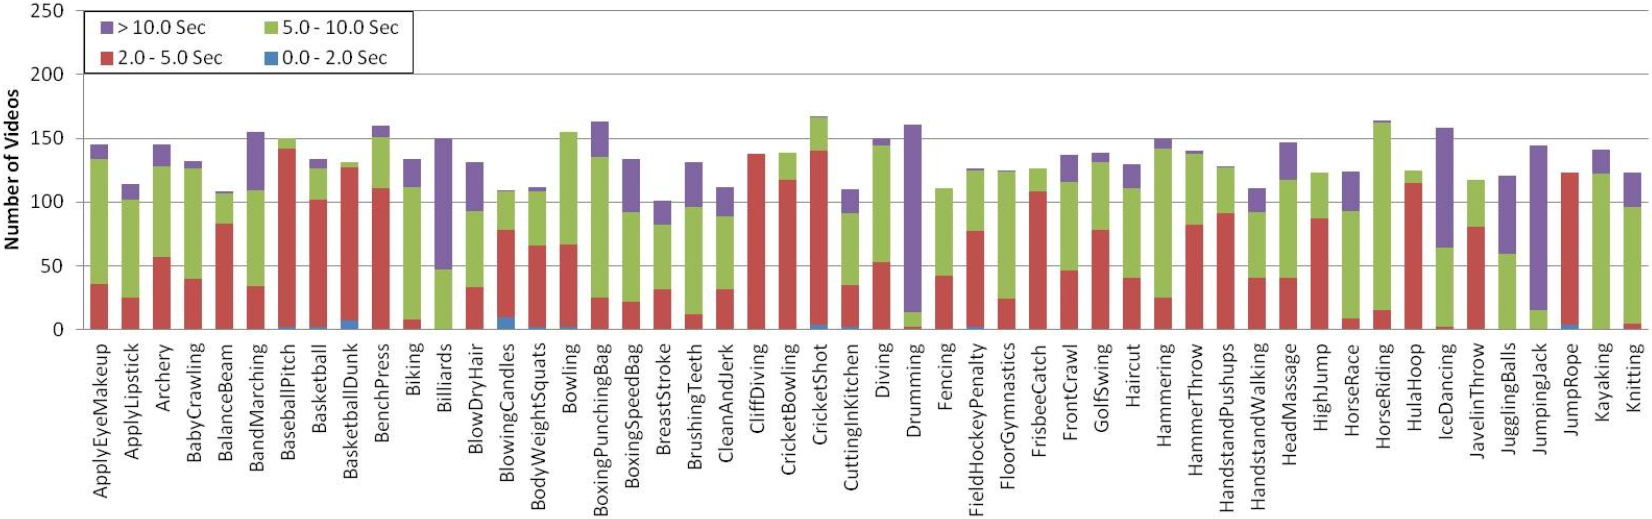
\includegraphics[width=0.8\textwidth]{101a.png}
	\caption{UCF101 Videos (1)}
	\label{101a}
\end{figure}
\begin{figure}[h]
	\centering
	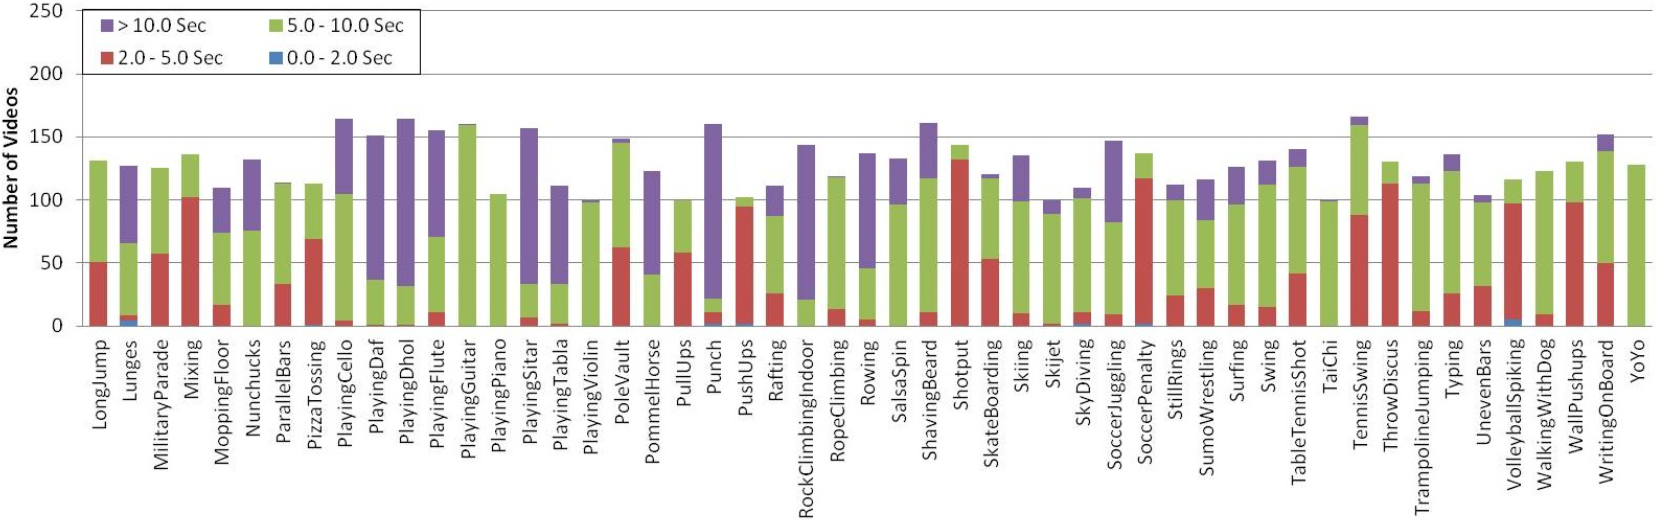
\includegraphics[width=0.8\textwidth]{101b.png}
	\caption{UCF101 Videos (2)}
	\label{101b}
\end{figure}
\\\indent aaaaaaaaaaaaaaaaaa Fig.\ref{frame}.
\begin{figure}[h]
	\centering
	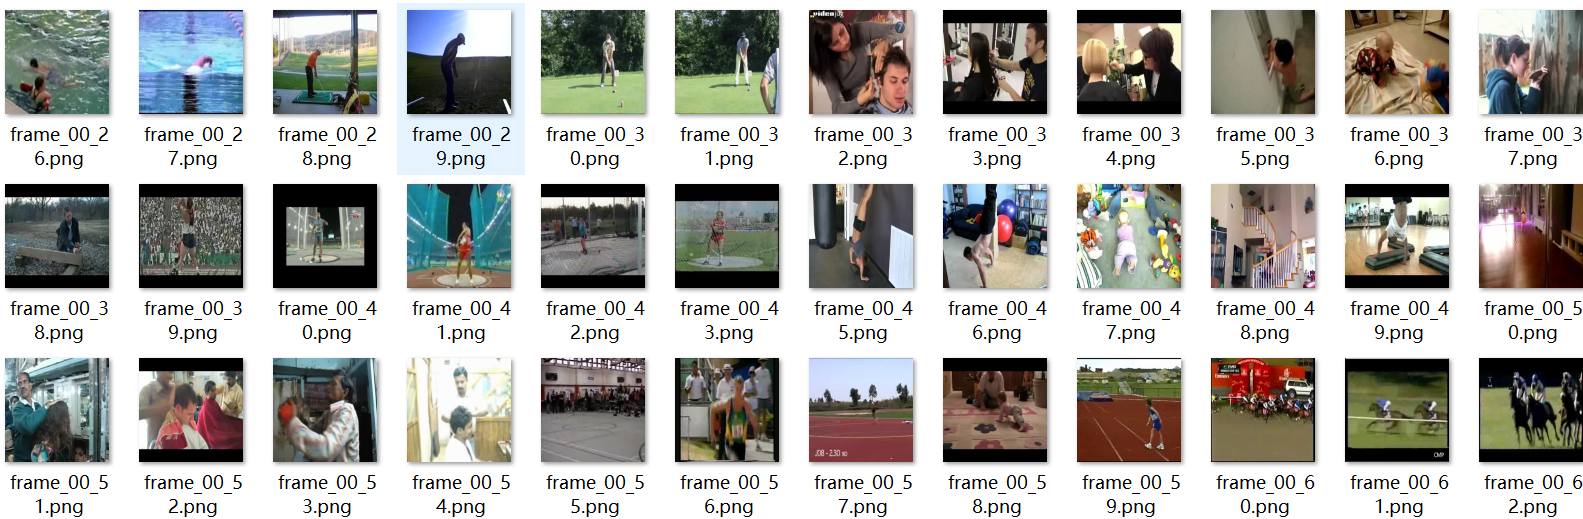
\includegraphics[width=0.8\textwidth]{frame.png}
	\caption{Keyframes of UCF101}
	\label{frame}
\end{figure}
\begin{figure}[h]
	\centering
	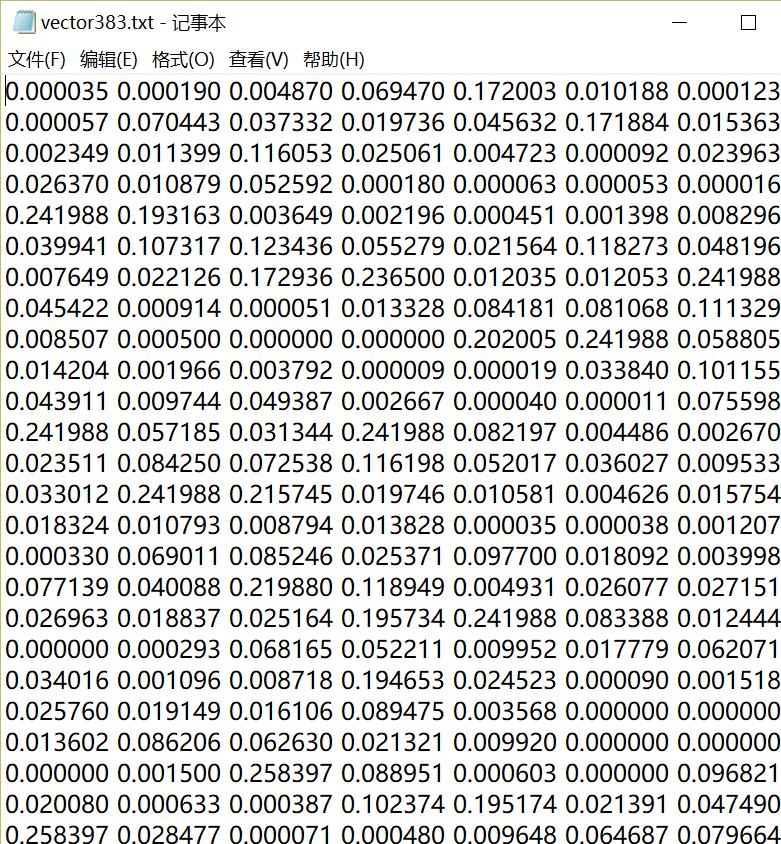
\includegraphics[width=0.4\textwidth]{vector1.png}
	\caption{Index of a Video}
	\label{vector1}
\end{figure}
\\\indent aaaaaaaaaaaa Fig.\ref{vector1}, \ref{vector2}. aaaaaaaaaaa
\begin{figure}[h]
	\centering
	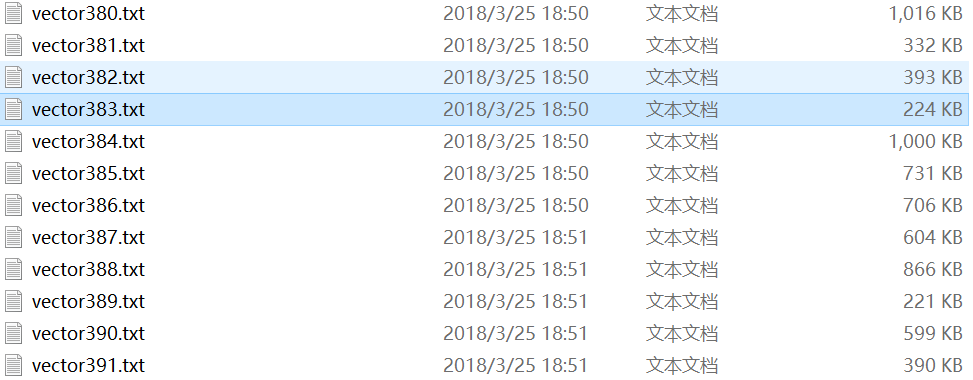
\includegraphics[width=0.9\textwidth]{vector2.png}
	\caption{Indexes of Videos}
	\label{vector2}
\end{figure}
\\\indent aaaaaaaaaaaaaaa 
\begin{figure}[h]
	\centering
	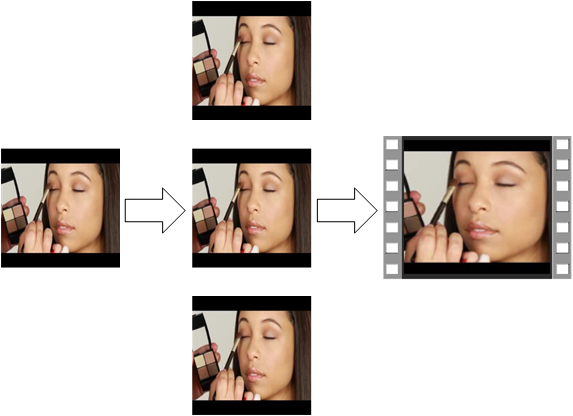
\includegraphics[width=0.71\textwidth]{search1.png}
	\caption{Search Results}
	\label{search1}
\end{figure}
\\\indent In the Fig.\ref{search1}, aaaaaaaaaaaaaaaa
\clearpage
\indent    %加个空格再clearpage就会制造空页,为了满足学校单双页要求 这里用newpage不行哦
\clearpage
\clearpage
\section{Conclusions and Outlook }
\setcounter{table}{0}  %保证每章节表标号从1开始
\setcounter{figure}{0} %保证每章节图片标号从1开始
\subsection{Conclusions}
In my final year project, I have implemented aaaaaaaa
\begin{itemize}
		\setlength{\itemsep}{1.50mm} %连续items之间的距离
		\setlength{\parskip}{0mm} %段落间的距离
		\setlength{\parsep}{0pt} %
		\item aaaaaaaa \cite{ye2017video},\cite{de2018semantic},\cite{DBLP:journals/tcsv/YinTZ18} aaaaaaaaaaaaa
		\item Secondly, aaaaaaaaaa
		\item aaaaa (\rmnum{1}) aaaaaaaaaa. (\rmnum{2}) aaaaaaaaaa
		\item aaaaaaaaa
\end{itemize}
\indent\indent aaaaaaa
\subsection{Reflection and Outlook}
In my three-month project for bachelor degree, aaaaaaaaaaaa
\\\indent(1) Read many papers in the field of information retrieval and searchable encryption.
\\\indent(2) Attend courses (Cryptography 1, Bitcoin and Cryptocurrency Technologies) on coursera.
\\\indent(3) Attend part of courses (Secure Software Engineering by Sherman S.M. CHOW, Cryptography by Andrej Bogdanov).
\\\indent(4) Implement a initial and acceptable searchable encryption scheme for videos.
\\\indent(5) Design a modified first-general-prototype after comparation, which enables searching and ranking related videos. 
\\\indent After my final-year project, I still have much needed works to complete this project finally. 
\\\indent(1) aaa
\\\indent(2) AAAA
%\section{Acknowlegement}
%\centering\includegraphics[width=0.99\textwidth]{zhixie.png}
%\centering\includegraphics[width=0.99\textwidth]{zhixiee.png}
\end{spacing}
\clearpage
\indent
\clearpage
\begin{spacing}{1.1}
	\newpage
	\small
	\bibliographystyle{ieeetr}
	\addcontentsline{toc}{section}{References}
	\bibliography{sample}
\end{spacing}
\clearpage
\indent
\clearpage
\rhead{\small ACKNOWLEDGEMENT}
\addcontentsline{toc}{section}{Acknowledgement}
\begin{center}
	\LARGE\textbf{Acknowledgement} 
\end{center}
\normalsize
\begin{spacing}{1.35}
注:本部分大致按时间顺序,无重要性区分。
\\\indent 岁月如梭,韶光易逝,四年的大学时光在不经意间悄悄溜走。致谢中文比较容易写出感情哦~
\\\indent 感谢aaaaaaaaaaaaaaaaaa
\\\indent 感谢aaaaaaaaa
\\\indent 感谢aaaaaaaaa
\\\indent 今当远离,不知所言;天涯海角,愿君安好;一路锋芒,一路辉煌。
\\
\\
\\\indent\indent\indent\indent\indent\indent\indent\indent\indent\indent\indent\indent 写于2018年5月20日凌晨
\end{spacing}
\clearpage
\rhead{\small ACHIEVEMENTS}
\begin{center}
	\LARGE\textbf{Achievements} 
\end{center}
\addcontentsline{toc}{section}{Achievements}
(1) 论文和专利 
\\\indent\rmnum{1}. Chong Fu, \textbf{Yu Zheng}, Min Chen, and Zhan-kao Wen. "A color image encryption algorithm using a new 1-D chaotic map", IEEE 17th International Conference on Communication Technology (ICCT), 2017. (Best Paper Award)
\\\indent\rmnum{2}. 付冲,\textbf{郑宇},何兴文.\ 一种具有与明文相关密钥流生成机制的混沌图像加密方法. (发明专利)
\\\indent(2) 研究和项目经历
\\\indent\rmnum{1}. 2018年3月 - 2018年5月
\\\indent Junior research assistant for searchable encryption supervised by Sherman S.M. CHOW.
\\\indent\rmnum{2}. 2016年8月 - 2017年4月
\\\indent 基于隐写术和混沌密码学的保密通信系统. (项目负责人,资助8.6万,大学生创新创业系列之重大项目)
\\\indent (3) 竞赛经历
\\\indent\rmnum{1}. 美国大学生数学建模大赛二等奖
\\\indent\rmnum{2}. 全国大学生数学建模大赛二等奖
\\\indent\rmnum{3}. 全国大学生信息安全竞赛三等奖
\\\indent\rmnum{4}. 辽宁省大学生数学建模大赛一等奖
\\\indent\rmnum{5}. 辽宁省大学生电子设计大赛二等奖

\end{document}